% ============================================================================
% Revised manuscript (DSP-D-26-02086)
%
% Pending results are marked with \tbd[...] and print in red. Before
% resubmission, search this file for "\tbd" and replace every occurrence:
%   1. Single-phase 1280 px, seed 42 (Table tab:schedule, abstract)
%   2. Stride control: YOLOv11s P3--P5, single phase 1280 px (Table tab:stride,
%      abstract, Sections 5.2 and 7). If the P2 level shows no gain, remove
%      "Detection Stride" from the title and revise Sections 3 and 7.
%   3. Size-stratified AP (Table tab:size)
%   4. UAVDT all-class evaluation (Table tab:uavdt, abstract)
%   5. FPS at 1280/1536 px on an idle GPU (Table tab:complexity)
%   6. Fraction of VisDrone training instances below 12.5 and 25 px
%      (Section 3; computed from dataset_stats.json, CPU only)
%   7. Declarations (CRediT roles, data availability, AI-use statement)
% ============================================================================

\documentclass[preprint,12pt]{elsarticle}

\usepackage{amsmath,amssymb}
\usepackage{graphicx}
\usepackage{xcolor}
\usepackage{booktabs}
\usepackage{multirow}
\usepackage{subcaption}
\usepackage{tikz}
\usetikzlibrary{positioning,arrows.meta,calc,backgrounds}
\usepackage{pgfplots}
\pgfplotsset{compat=1.17}
\usepackage{hyperref}
\hypersetup{colorlinks=true, linkcolor=blue, citecolor=blue, urlcolor=blue}

% Colour-blind-safe palette (Okabe--Ito)
\definecolor{cSP}{HTML}{0072B2}     % single-phase training
\definecolor{cProg}{HTML}{E69F00}   % progressive training
\definecolor{cMod}{HTML}{D55E00}    % feature modules
\definecolor{cGreen}{HTML}{009E73}  % detection heads
\definecolor{cObj}{HTML}{D55E00}    % objects in schematics

\pgfplotsset{
  every axis/.append style={
    font=\footnotesize,
    tick label style={font=\scriptsize},
    label style={font=\footnotesize},
    legend style={font=\scriptsize},
  },
}

% Placeholder for results that are still being computed
\newcommand{\tbd}[1][TBD]{\textcolor{red}{\textbf{[#1]}}}

\journal{Digital Signal Processing}

\begin{document}

\begin{frontmatter}

\title{What Drives Small Object Detection Accuracy in UAV Imagery?\\
A Controlled Study of Training Resolution, Detection Stride, and Feature Modules}

\author[zjnu]{Moatassim Barakat}
\author[zjnu]{Xinzhong Zhu\corref{cor1}}
\ead{zxz@zjnu.edu.cn}
\cortext[cor1]{Corresponding author.}

\affiliation[zjnu]{
    organization={College of Computer Science and Technology,
                  Zhejiang Normal University},
    addressline={688 Yingbin Road},
    city={Jinhua},
    postcode={321004},
    country={China}
}

\begin{abstract}
Small-object detectors for drone imagery are often built by attaching modules to
a YOLO baseline, with gains of one to three points usually measured in a single
training run. We asked which design decisions still matter once the training
budget, evaluation settings and random seed are controlled. Using YOLOv11s on
VisDrone-DET2019, we compared a four-phase progressive resolution schedule with
single-resolution training at the same epoch budget, added a stride-4 detection
level, and tested multi-scale edge information selection (MEIS), cross-scale
weighted fusion and CBAM-style recalibration. Differences were tested with paired
image-level bootstrap and permutation tests.
Training at 1280\,px in a single phase outperformed the progressive schedule by
3.9 points mAP@50 at 1280\,px (57.3\% vs.\ 53.3\%, $p<0.001$) and matched the
schedule's final accuracy after one third of its compute. MEIS with recalibration
changed mAP@50 by $+0.6$ and $-0.3$ points on two seeds, neither significant, and
a reduced-budget factorial ablation found no benefit from multi-scale dilation or
input-adaptive gating over a plain convolution of the same size. The stride-4
level changed mAP@50 by \tbd[X] points. We explain these results with a sampling
argument: input scale and feature stride fix how many anchor points fall on a
small object, and modules that act after downsampling cannot add them back. The
best configuration reaches 58.8\% mAP@50 at 1536\,px with 9.9M parameters. On
UAVDT, which contains only vehicles, \tbd[UAVDT result]; generalization to small
non-vehicle objects outside VisDrone is untested.
\end{abstract}

\begin{highlights}
\item Single-resolution training beat a four-phase resolution curriculum by 3.9 pp
\item It matched the curriculum's final accuracy using a third of the compute
\item Edge selection and CBAM-style recalibration gave no significant gain
\item Neither multi-scale dilation nor adaptive gating beat a plain convolution
\item Input scale and stride set how many anchor points fall on a small object
\end{highlights}

\begin{keyword}
Small object detection \sep UAV imagery \sep Sampling resolution \sep
Training schedule \sep Ablation study \sep Statistical significance \sep YOLOv11
\end{keyword}

\end{frontmatter}

% ============================================================================
\section{Introduction}
\label{sec:intro}
% ============================================================================

Drones photograph scenes from tens to hundreds of metres above the ground, so the
objects that matter for traffic monitoring, crowd counting or search and rescue
often cover only a few dozen pixels~\cite{visdrone2019,uav-survey}. In the
VisDrone-DET2019 training set, 63\% of the annotated instances have a
geometric-mean side shorter than 32 pixels in the original frame. After the
frame is resized for the network, such an object falls on a handful of cells of
a stride-8 feature map, and a detector that sees only a few samples of an object
has little to work with, however its later layers are designed.

Much of the recent work on this problem modifies the network. Attention blocks,
edge enhancement branches, weighted feature fusion and extra prediction heads
have all been attached to YOLO baselines~\cite{tph-yolo,meis-yolo,cf-yolo}, and
the reported improvements are usually modest; MEIS-YOLO, for example, reports
1.4 points of AP@50 over its YOLOv11 baseline~\cite{meis-yolo}. Two things make
gains of that size hard to interpret. If the proposed model and its baseline are
not trained under the same conditions, a gain that comes from a longer schedule
or a larger input can end up credited to the new module. And networks trained
from different random seeds reach different
accuracies~\cite{bouthillier2021variance}; for detectors on VisDrone we measured
seed-to-seed differences of up to 0.7 points, which is comparable to the effects
being claimed.

This paper reports what happened when we removed those confounds. We started from
YOLOv11s~\cite{yolov11} and three modules that target the usual explanations for
poor small-object accuracy: a multi-scale edge information selection (MEIS) block
built from dilated depthwise-separable branches with input-adaptive gating,
following the idea of MEIS-YOLO~\cite{meis-yolo}; a cross-scale weighted fusion
neck in the spirit of CF-YOLO~\cite{cf-yolo} and BiFPN~\cite{efficientdet}; and a
CBAM-style recalibration module~\cite{cbam} placed after fusion. We also studied
two changes that act on sampling rather than on features: the input resolution
used for training, reached either directly or through a four-phase progressive
schedule, and a stride-4 (P2) detection level. Every comparison uses a matched
epoch budget and one evaluation protocol, and each was repeated with independent
seeds and tested with paired resampling over the validation images.

The results did not follow the module-centred story we expected. Single-resolution
training at 1280\,px was 3.9 points better than the progressive schedule at the
same epoch budget, and it reached the schedule's final accuracy with one third of
its compute. MEIS with recalibration produced no significant change on either of
two seeds. A factorial ablation showed that neither of the two ingredients that
define MEIS, multi-scale dilation and input-adaptive gating, did better than a
plain convolution with the same number of parameters. The stride-4 level
\tbd[summarise stride result]. This pattern is what one would expect if accuracy
on small objects is limited mainly by how densely each object is sampled, and
Section~\ref{sec:sampling} makes that argument concrete for anchor-free detectors.

The paper makes three contributions: (i)~a matched-budget comparison of
progressive and single-resolution training for small-object detection, with
measured compute and paired significance tests; (ii)~a controlled evaluation of
edge selection, weighted fusion and recalibration modules, including a factorial
ablation that separates multi-scale dilation, adaptive gating and added capacity;
and (iii)~a sampling account of these results that gives, for a given input size
and stride, the smallest object that can receive positive training samples.

% ============================================================================
\section{Related Work}
\label{sec:related}
% ============================================================================

\subsection{Feature modules for small aerial objects}

Feature pyramids~\cite{fpn,panet} and weighted bidirectional
fusion~\cite{efficientdet} are the standard way to give a detector features at
several scales, and channel or spatial attention~\cite{senet,cbam,ecanet} is
often added to suppress the cluttered backgrounds of aerial scenes. Detectors
designed for drone imagery combine these ideas. TPH-YOLOv5~\cite{tph-yolo} adds
transformer prediction heads, CBAM and an extra prediction head for tiny objects.
MEIS-YOLO~\cite{meis-yolo} inserts an edge information selection block, an
asymptotic feature pyramid and bi-level routing attention into YOLOv11.
CF-YOLO~\cite{cf-yolo} replaces the YOLOv5s neck with cross-fusion blocks for
detection in snow. These papers report their gains without estimates of
run-to-run variation, which makes differences of a point or two difficult to
judge. When a design adds a higher-resolution head together with new blocks, as
TPH-YOLOv5 does, the change in sampling alone may account for part of the gain.

\subsection{Resolution and sampling in aerial detection}

A second line of work treats small objects as a resolution problem. Coarse-to-fine
detectors such as ClusDet~\cite{clusdet}, DMNet~\cite{li2020dmnet} and
UFPMP-Det~\cite{huang2022ufpmp} locate object-dense regions and process them at
higher magnification. QueryDet~\cite{yang2022querydet} runs a cheap coarse pass
and computes high-resolution features only where small objects are likely, and
SAHI~\cite{akyon2022sahi} slices large images into overlapping tiles. These
methods show that magnification helps, but they also change the inference pipeline
and its cost. We look at the two simplest sampling controls available inside a
single-pass detector: the input resolution used in training and the stride of the
finest detection level.

\subsection{Resolution schedules during training}

Curriculum learning~\cite{curriculum-learning} orders training from easy to hard,
and progressive resizing applies a similar idea to image resolution.
EfficientNetV2~\cite{tan2021efficientnetv2} trains image classifiers on small
images first and raises resolution and regularization together, mainly to shorten
training. Touvron et al.~\cite{touvron2019fixres} showed that test-time resolution
interacts with training resolution, so a classifier can benefit from being tested
at a larger size than it was trained on. Both lines of work concern
classification. For dense detection of tiny objects, where a low training
resolution can shrink objects below the size a detection level can represent, we
are not aware of a matched-budget comparison between progressive and
single-resolution training.

\subsection{Variance and significance in detector evaluation}

Networks trained with different seeds, data orders and initializations reach
different accuracies, and Bouthillier et al.~\cite{bouthillier2021variance} showed
that ignoring this variation leads to unreliable conclusions in machine learning
benchmarks. When a metric is computed over a test set, paired resampling
tests~\cite{efron1993bootstrap,bergkirkpatrick2012significance} offer a practical
check, because both models are scored on the same resampled images. Detection
papers rarely report them. We apply them at the image level and report separately
how much results move between seeds.

% ============================================================================
\section{A Sampling View of Small Object Detection}
\label{sec:sampling}
% ============================================================================

A detector does not see an object at its original size. A frame whose longer side
is $W_0$ pixels is resized so that this side equals the network input size $S$,
which scales an object of side $a$ to $ka$ with $k=S/W_0$. A feature level with
stride $r$ then samples the resized image once every $r$ pixels, so the number of
samples across the object is
\begin{equation}
  n = \frac{k\,a}{r} = \frac{S\,a}{r\,W_0}.
  \label{eq:samples}
\end{equation}
Seen as a sampling problem, $n$ is the sampling rate relative to the object.
With fewer than about two samples per side, a level cannot represent the object's
spatial structure, and the layers that follow inherit the
loss~\cite{shannon1949communication,zhang2019antialiased}.

For anchor-free YOLO detectors the consequence is more direct. YOLOv11 assigns
training targets with the task-aligned assigner of TOOD~\cite{feng2021tood}, which
only considers anchor points whose centres lie inside a ground-truth box. At a
given level an object covers roughly $n_w n_h$ anchor points, where $n_w$ and
$n_h$ count samples along its width and height. When both counts are below one,
the object may contain no anchor point at that level. If that happens at every
level, the object contributes no positive sample and is learned only as
background. Setting $n$ to one or two in Eq.~\eqref{eq:samples} gives the smallest
object side that can be assigned a target, and the smallest that is sampled twice
per side:
\begin{equation}
  a_{\min} = \frac{n\, r\, W_0}{S}.
  \label{eq:amin}
\end{equation}
Fig.~\ref{fig:sampling} illustrates the effect and Table~\ref{tab:amin} evaluates
Eq.~\eqref{eq:amin} for frames 2000 pixels wide, which is about the size of the
largest VisDrone-DET2019 frames. Halving the stride and doubling the input size
have the same effect on $a_{\min}$. At an input size of 640\,px a stride-8 level
cannot assign targets to objects smaller than 25 pixels, a range that contains
\tbd[X]\% of the VisDrone training instances; at 1280\,px with a stride-4 level
the threshold drops to 6.3 pixels (\tbd[Y]\% of instances below it).

\begin{figure}[t]
\centering
\resizebox{\linewidth}{!}{%
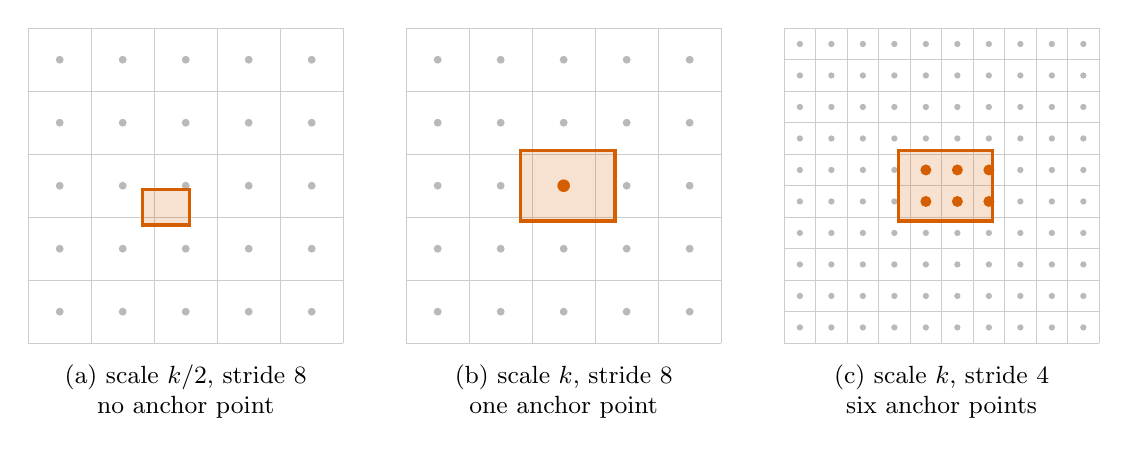
\begin{tikzpicture}[x=1cm,y=1cm]
  \tikzset{
    anch/.style={fill=gray!55},
    hit/.style={fill=cObj},
    obj/.style={draw=cObj, very thick, fill=cObj, fill opacity=0.18},
    lbl/.style={align=center, font=\small, anchor=north},
  }
  % (a) half input scale, stride 8
  \begin{scope}
    \draw[step=0.8, gray!40] (0,0) grid (4,4);
    \foreach \i in {0,...,4} { \foreach \j in {0,...,4} {
      \fill[anch] ({0.4+0.8*\i},{0.4+0.8*\j}) circle (0.05); } }
    \draw[obj] (1.45,1.50) rectangle (2.05,1.95);
    \node[lbl] at (2,-0.15) {(a) scale $k/2$, stride 8\\no anchor point};
  \end{scope}
  % (b) full input scale, stride 8
  \begin{scope}[xshift=4.8cm]
    \draw[step=0.8, gray!40] (0,0) grid (4,4);
    \foreach \i in {0,...,4} { \foreach \j in {0,...,4} {
      \fill[anch] ({0.4+0.8*\i},{0.4+0.8*\j}) circle (0.05); } }
    \draw[obj] (1.45,1.55) rectangle (2.65,2.45);
    \fill[hit] (2.0,2.0) circle (0.08);
    \node[lbl] at (2,-0.15) {(b) scale $k$, stride 8\\one anchor point};
  \end{scope}
  % (c) full input scale, stride 4
  \begin{scope}[xshift=9.6cm]
    \draw[step=0.4, gray!40] (0,0) grid (4,4);
    \foreach \i in {0,...,9} { \foreach \j in {0,...,9} {
      \fill[anch] ({0.2+0.4*\i},{0.2+0.4*\j}) circle (0.04); } }
    \draw[obj] (1.45,1.55) rectangle (2.65,2.45);
    \foreach \x in {1.8,2.2,2.6} { \foreach \y in {1.8,2.2} {
      \fill[hit] (\x,\y) circle (0.07); } }
    \node[lbl] at (2,-0.15) {(c) scale $k$, stride 4\\six anchor points};
  \end{scope}
\end{tikzpicture}%
}
\caption{The same object (red box) under three sampling settings. Grid cells span
one stride in network-input pixels and dots mark anchor points; filled red dots
lie inside the object and can be assigned as positive samples. Halving the input
scale (a) removes the only anchor point that the object covers at stride 8 (b),
while a stride-4 level (c) places six anchor points on it.}
\label{fig:sampling}
\end{figure}

\begin{table}[t]
\centering
\caption{Smallest object side $a_{\min}$, in pixels of a 2000-pixel-wide frame,
that yields at least $n$ anchor points per side (Eq.~\ref{eq:amin}).}
\label{tab:amin}
\small
\begin{tabular}{llrrrrr}
\toprule
 & & \multicolumn{5}{c}{Network input size $S$ (px)} \\
\cmidrule(lr){3-7}
Stride $r$ & $n$ & 640 & 800 & 1024 & 1280 & 1536 \\
\midrule
4 (P2) & 1 & 12.5 & 10.0 &  7.8 &  6.3 &  5.2 \\
       & 2 & 25.0 & 20.0 & 15.6 & 12.5 & 10.4 \\
\addlinespace
8 (P3) & 1 & 25.0 & 20.0 & 15.6 & 12.5 & 10.4 \\
       & 2 & 50.0 & 40.0 & 31.3 & 25.0 & 20.8 \\
\bottomrule
\end{tabular}
\end{table}

The argument leads to three predictions that the experiments can check.
\begin{enumerate}
  \item[P1.] Training at a larger input size, or adding a finer detection level,
  should help most on small objects, because both raise $n$ for the same frames.
  \item[P2.] A module that operates on stride-$r$ features cannot raise $n$. It can
  reweight what was sampled, but it cannot give training signal to objects that
  received no positive samples.
  \item[P3.] A progressive schedule that starts at low resolution spends its early
  epochs in a regime where many small objects cannot be assigned targets
  (Table~\ref{tab:amin}, 640 and 800\,px). Under a fixed epoch budget it should
  therefore do worse than training at the final resolution throughout.
\end{enumerate}
Eq.~\eqref{eq:amin} is a simplification. Mosaic and scale augmentation change $k$
from one training image to the next, context around an object can support
detection, and the assigner's behaviour near box borders depends on implementation
details. We use the argument to organise the experiments, not as a quantitative
model of accuracy.

% ============================================================================
\section{Experimental Setup}
\label{sec:setup}
% ============================================================================

\subsection{Dataset}

We use VisDrone-DET2019~\cite{visdrone2019}, which provides 6,471 training images
and 548 validation images annotated with ten object categories. All results in
this paper are on the validation set; we did not use the test-dev split.
Annotations were converted to the YOLO format, keeping categories 1 to 10 and
discarding ignored regions (category~0) and the \emph{others} class (category~11).
Boxes were clipped to the image, and boxes one pixel wide or high or smaller after
clipping were removed. The converted training set contains 305,974 instances and
the validation set 38,759. The class distribution is strongly skewed
(Fig.~\ref{fig:classes}): cars and pedestrians account for 65.5\% of training
instances, while tricycles, awning-tricycles and buses together make up 4.3\%.

\begin{figure}[t]
\centering
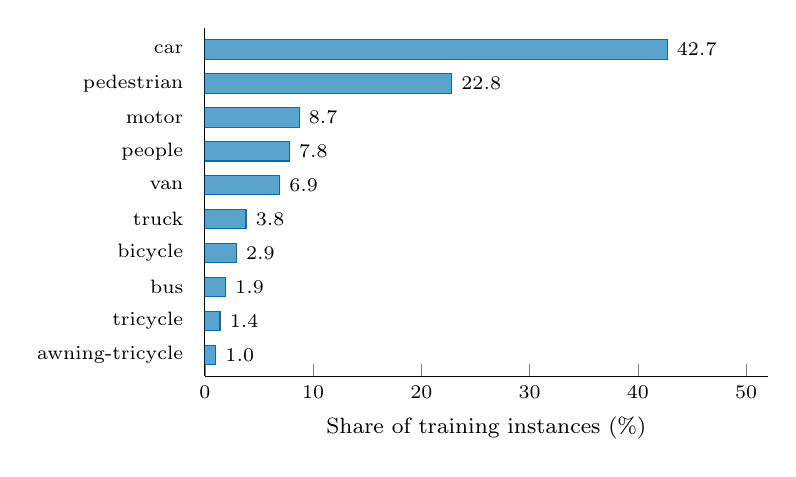
\begin{tikzpicture}
\begin{axis}[
  xbar, width=0.72\linewidth, height=6.0cm, bar width=7pt,
  xmin=0, xmax=52, xlabel={Share of training instances (\%)},
  ytick={1,...,10},
  yticklabels={awning-tricycle, tricycle, bus, bicycle, truck, van, people,
               motor, pedestrian, car},
  enlarge y limits=0.07,
  nodes near coords={\pgfmathprintnumber[fixed,precision=1,fixed zerofill]{\pgfplotspointmeta}},
  point meta=x,
  nodes near coords style={font=\scriptsize, anchor=west},
  axis x line*=bottom, axis y line*=left, ytick style={draw=none},
]
\addplot[fill=cSP!65, draw=cSP] coordinates {
  (1.0,1) (1.4,2) (1.9,3) (2.9,4) (3.8,5) (6.9,6) (7.8,7) (8.7,8) (22.8,9) (42.7,10)};
\end{axis}
\end{tikzpicture}
\caption{Class distribution of the 305,974 training instances in VisDrone-DET2019
after conversion.}
\label{fig:classes}
\end{figure}

\subsection{Detectors and modules}
\label{sec:models}

All detectors are built on YOLOv11s~\cite{yolov11} and initialized from its
COCO-pretrained weights. The stock model detects at strides 8, 16 and 32 (P3 to
P5). The \emph{Baseline-P2} variant extends the top-down path of the neck to the
stride-4 backbone features and starts the bottom-up path from there, which gives
four detection levels (Fig.~\ref{fig:arch}). Where a modified neck contains C3k2
blocks whose weight shapes match the original head, those weights are copied as
well, so that no variant starts from a randomly initialized block when a
pretrained counterpart exists.

\begin{figure}[t]
\centering
\resizebox{\linewidth}{!}{%
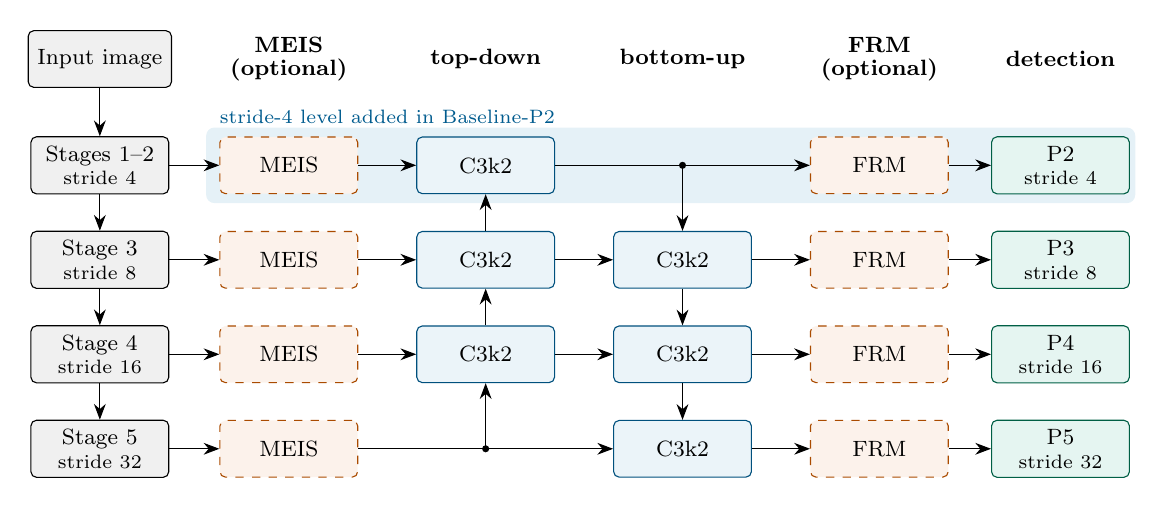
\begin{tikzpicture}[
  font=\footnotesize, >={Stealth[length=2mm]},
  blk/.style={draw, rounded corners=2pt, minimum width=1.75cm,
              minimum height=0.72cm, align=center, fill=white},
  bb/.style={blk, fill=gray!12},
  neck/.style={blk, fill=cSP!8, draw=cSP!70!black},
  opt/.style={blk, dashed, draw=cMod!80!black, fill=cMod!8},
  head/.style={blk, fill=cGreen!10, draw=cGreen!60!black},
  lab/.style={font=\footnotesize\bfseries, align=center},
]
  \begin{scope}[on background layer]
    \fill[cSP!10, rounded corners=3pt] (1.35,2.52) rectangle (13.15,3.48);
  \end{scope}
  % column labels
  \node[bb]  (in) at (0,4.35) {Input image};
  \node[lab] at (2.4,4.35) {MEIS\\[-1pt](optional)};
  \node[lab] at (4.9,4.35) {top-down};
  \node[lab] at (7.4,4.35) {bottom-up};
  \node[lab] at (9.9,4.35) {FRM\\[-1pt](optional)};
  \node[lab] at (12.2,4.35) {detection};
  % backbone
  \node[bb] (b2) at (0,3.0)  {Stages 1--2\\[-1pt]\scriptsize stride 4};
  \node[bb] (b3) at (0,1.8)  {Stage 3\\[-1pt]\scriptsize stride 8};
  \node[bb] (b4) at (0,0.6)  {Stage 4\\[-1pt]\scriptsize stride 16};
  \node[bb] (b5) at (0,-0.6) {Stage 5\\[-1pt]\scriptsize stride 32};
  % optional MEIS
  \node[opt] (m2) at (2.4,3.0)  {MEIS};
  \node[opt] (m3) at (2.4,1.8)  {MEIS};
  \node[opt] (m4) at (2.4,0.6)  {MEIS};
  \node[opt] (m5) at (2.4,-0.6) {MEIS};
  % neck
  \node[neck] (t2) at (4.9,3.0) {C3k2};
  \node[neck] (t3) at (4.9,1.8) {C3k2};
  \node[neck] (t4) at (4.9,0.6) {C3k2};
  \node[neck] (u3) at (7.4,1.8)  {C3k2};
  \node[neck] (u4) at (7.4,0.6)  {C3k2};
  \node[neck] (u5) at (7.4,-0.6) {C3k2};
  % optional FRM
  \node[opt] (f2) at (9.9,3.0)  {FRM};
  \node[opt] (f3) at (9.9,1.8)  {FRM};
  \node[opt] (f4) at (9.9,0.6)  {FRM};
  \node[opt] (f5) at (9.9,-0.6) {FRM};
  % heads
  \node[head] (h2) at (12.2,3.0)  {P2\\[-1pt]\scriptsize stride 4};
  \node[head] (h3) at (12.2,1.8)  {P3\\[-1pt]\scriptsize stride 8};
  \node[head] (h4) at (12.2,0.6)  {P4\\[-1pt]\scriptsize stride 16};
  \node[head] (h5) at (12.2,-0.6) {P5\\[-1pt]\scriptsize stride 32};
  % backbone flow
  \draw[->] (in) -- (b2);
  \draw[->] (b2) -- (b3);
  \draw[->] (b3) -- (b4);
  \draw[->] (b4) -- (b5);
  \foreach \i in {2,3,4,5} { \draw[->] (b\i) -- (m\i); }
  % top-down path
  \draw[->] (m5.east) -| (t4.south);
  \draw[->] (m4) -- (t4);
  \draw[->] (t4) -- (t3);
  \draw[->] (m3) -- (t3);
  \draw[->] (t3) -- (t2);
  \draw[->] (m2) -- (t2);
  % bottom-up path
  \draw[->] (t2.east) -- (f2.west);
  \draw[->] (t2.east) -| (u3.north);
  \draw[->] (t3) -- (u3);
  \draw[->] (u3) -- (u4);
  \draw[->] (t4) -- (u4);
  \draw[->] (u4) -- (u5);
  \draw[->] (m5.east) -- (u5.west);
  \fill (7.4,3.0) circle (0.045);
  \fill (4.9,-0.6) circle (0.045);
  % outputs
  \draw[->] (u3) -- (f3);
  \draw[->] (u4) -- (f4);
  \draw[->] (u5) -- (f5);
  \foreach \i in {2,3,4,5} { \draw[->] (f\i) -- (h\i); }
  \node[font=\scriptsize, text=cSP!80!black, anchor=west] at (1.4,3.62)
    {stride-4 level added in Baseline-P2};
\end{tikzpicture}%
}
\caption{Detector variants. The Baseline-P2 neck extends the YOLOv11s path
aggregation neck to the stride-4 backbone features (shaded row). Each C3k2 node in
the top-down path follows an upsampling and concatenation, and each node in the
bottom-up path follows a strided convolution and concatenation. Dashed blocks are
the optional modules evaluated in Section~\ref{sec:res-modules}; Stage~5 includes
the SPPF and C2PSA blocks of YOLOv11.}
\label{fig:arch}
\end{figure}

\paragraph{Multi-scale edge information selection (MEIS)}
MEIS is applied to each backbone output that feeds the neck. For an input
$X\in\mathbb{R}^{C\times H\times W}$, three depthwise-separable branches with
dilation $d\in\{1,2,4\}$ produce edge responses $E_d$, and a channel gate computed
from each response weights it:
\begin{equation}
  g_d = \sigma\!\big(W_2\,\delta(W_1\,\mathrm{GAP}(E_d))\big)\in[0,1]^C, \qquad
  Y = X + \sum_{d} g_d \odot E_d ,
  \label{eq:meis}
\end{equation}
where $\mathrm{GAP}$ is global average pooling, $W_1$ and $W_2$ are $1{\times}1$
convolutions with reduction ratio 16, $\delta$ is ReLU and $\sigma$ the sigmoid.
The gate is recomputed for every input. Our block tests the dilation-and-gating
interpretation of edge selection; the MEIS module of MEIS-YOLO~\cite{meis-yolo}
instead uses adaptive pooling, high-pass edge enhancement and a dual-domain
selection mechanism, so our results do not transfer to that module directly.

\paragraph{Feature recalibration module (FRM)}
FRM applies the channel and spatial attention of CBAM~\cite{cbam} to each neck
output and blends the result residually,
$Y = X + \alpha\,(X_c - X) + \alpha\,(X_s - X_c)$, where $X_c$ and $X_s$ are the
outputs of the channel and spatial attention steps and $\alpha=0.5$.

\paragraph{Factorial variants}
To separate the ingredients of MEIS, we replaced the dilations $(1,2,4)$ with
$(1,1,1)$, which leaves the parameter count unchanged, and replaced the
input-adaptive gate with an input-independent learnable channel weight
$\sigma(\theta_d)$, $\theta_d\in\mathbb{R}^C$. The weights $\theta_d$ are
initialized to zero, so both gate types start close to 0.5. The variant with
dilations $(1,1,1)$ and a static gate is a plain residual block of
depthwise-separable convolutions with the same capacity as MEIS and no multi-scale
or adaptive component.

\paragraph{Cross-scale weighted fusion}
This neck, evaluated only in the earlier experiments of Appendix~\ref{app:early},
combines resized and channel-projected pyramid features $\tilde F_i$ with
normalized learnable weights,
$F = \sum_i \frac{\mathrm{ReLU}(w_i)}{\sum_j \mathrm{ReLU}(w_j)+\epsilon}\,\tilde F_i$,
followed by a depthwise-separable convolution, similar to the fast normalized
fusion of BiFPN~\cite{efficientdet}.

Table~\ref{tab:complexity} lists the size and computational cost of each variant.

\begin{table}[t]
\centering
\caption{Parameters, computational cost and speed of the evaluated detectors.}
\label{tab:complexity}
\small
\resizebox{\linewidth}{!}{%
\begin{tabular}{lcrrrrrr}
\toprule
 & & & \multicolumn{3}{c}{GFLOPs at input size} & \multicolumn{2}{c}{FPS at input size} \\
\cmidrule(lr){4-6}\cmidrule(lr){7-8}
Model & Levels & Params (M) & 640 & 1280 & 1536 & 1280 & 1536 \\
\midrule
YOLOv11s (P3--P5)                    & 3 &  9.43 & 21.6 &  86.3 & 124.2 & \tbd & \tbd \\
Baseline-P2                          & 4 &  9.92 & 37.5 & 149.8 & 215.7 & \tbd & \tbd \\
Baseline-P2 + MEIS + FRM             & 4 & 11.40 & 44.4 & 177.4 & 255.5 & \tbd & \tbd \\
\quad dilation (1,1,1), adaptive gate & 4 & 11.40 & 44.4 & 177.4 & 255.5 & -- & -- \\
\quad dilation (1,2,4), static gate   & 4 & 11.25 & 44.3 & 177.3 & 255.3 & -- & -- \\
\quad dilation (1,1,1), static gate   & 4 & 11.25 & 44.3 & 177.3 & 255.3 & -- & -- \\
\bottomrule
\end{tabular}%
}
\\[2pt]
\begin{minipage}{\linewidth}\footnotesize
GFLOPs are twice the multiply--accumulate operations for one square image with
unfused convolution and batch-normalization layers. FPS: one NVIDIA RTX~3080,
batch size 1, FP16, network forward pass only.
\end{minipage}
\end{table}

\subsection{Training}
\label{sec:training}

Table~\ref{tab:schedules} lists the two schedules. The \emph{progressive} schedule
trains for 100, 100, 100 and 50 epochs at 640, 800, 1024 and 1280\,px. Each phase
restarts a cosine learning-rate schedule with warm-up, and augmentation strength
decreases while the box and classification loss weights increase from phase to
phase. The \emph{single-phase} schedule trains for all 350 epochs at 1280\,px with
the phase-1 settings. Both use SGD with momentum 0.937 and weight decay
$5\times10^{-4}$, mixed precision, and the exponential moving average of weights
provided by the Ultralytics trainer. Batch sizes were limited by the memory needed
for the P2 models at 1280\,px and were the same for every model trained with a
given schedule.

\begin{table}[t]
\centering
\caption{Training schedules. Learning rates follow a cosine curve from lr$_0$ to
lr$_0\cdot f$ within each phase.}
\label{tab:schedules}
\footnotesize
\resizebox{\linewidth}{!}{%
\begin{tabular}{lrrrllrlll}
\toprule
 & Input & Epochs & Batch & lr$_0$ & $f$ & Warm-up & Loss weights & Mosaic / mixup & Scale / \\
 & (px) & & & & & (ep.) & box / cls / DFL & / copy-paste & rotation \\
\midrule
Progressive, phase 1 &  640 & 100 & 8 & 0.01   & 0.01 & 5 & 7.5 / 0.5 / 1.5 & 1.0 / 0.15 / 0.3 & 0.9 / 10$^\circ$ \\
Progressive, phase 2 &  800 & 100 & 6 & 0.005  & 0.05 & 3 & 8.0 / 0.6 / 1.6 & 0.8 / 0.10 / 0.4 & 0.8 / 7$^\circ$ \\
Progressive, phase 3 & 1024 & 100 & 4 & 0.002  & 0.08 & 2 & 8.5 / 0.7 / 1.7 & 0.5 / 0.05 / 0.2 & 0.7 / 5$^\circ$ \\
Progressive, phase 4 & 1280 &  50 & 2 & 0.0005 & 0.10 & 1 & 9.0 / 0.8 / 1.8 & 0 / 0 / 0.1       & 0.6 / 2$^\circ$ \\
\midrule
Single phase         & 1280 & 350 & 2 & 0.01   & 0.01 & 5 & 7.5 / 0.5 / 1.5 & 1.0 / 0.15 / 0.3 & 0.9 / 10$^\circ$ \\
\bottomrule
\end{tabular}%
}
\\[2pt]
\begin{minipage}{\linewidth}\footnotesize
Mosaic augmentation is switched off for the last 20, 15, 10 and 0 epochs of phases
1--4, and for the last 20 epochs of the single-phase schedule.
\end{minipage}
\end{table}

We report training compute in pixel-epochs, $C=\sum_{e} S_e^2$, the sum over
epochs of the squared input size. Convolutional cost grows with the number of
input pixels, so $C$ compares schedules independently of hardware and of other
jobs sharing the machine. The progressive schedule costs $2.92\times10^{8}$
pixel-epochs and 350 epochs at 1280\,px cost $5.73\times10^{8}$.

Each configuration was trained with seeds 0 and 42. The factorial ablation of
Section~\ref{sec:res-factorial} used a shortened progressive schedule with 25,
20, 20 and 10 epochs per phase and was otherwise identical. Experiments ran on
NVIDIA RTX~3080 GPUs (20\,GB) with Ultralytics~8.4, PyTorch~2.5.1 and CUDA~12.1.

\subsection{Evaluation}

All models were evaluated with the Ultralytics validator using letterbox resizing
to input size $S$, a confidence threshold of 0.001, non-maximum suppression at an
IoU of 0.5 and at most 600 detections per image. The validation images contain
70.7 annotated instances on average. We report mAP@50 and mAP@50:95 with
101-point interpolation, and precision and recall at the confidence threshold that
maximizes the mean F1 score. The primary input size is 1280\,px, the final
training resolution of both schedules; we also report 1536\,px.

\subsection{Statistical testing}
\label{sec:stats}

Differences between two models were tested on the 548 validation images with two
paired procedures. Per-image detection statistics were captured from the validator
with batch size one, and recomputing mAP from them reproduces the validator's
reported value. In the \emph{paired bootstrap}~\cite{efron1993bootstrap}, the
images were resampled with replacement 1000 times, both models were scored on each
resample, and the 2.5th and 97.5th percentiles of the difference form the 95\%
confidence interval. The two-sided $p$-value is twice the smaller fraction of
resampled differences lying on either side of zero; when no resample crosses zero
we report $p<0.001$. In the \emph{paired permutation test}, the two models'
statistics were swapped independently for each image with probability 0.5, 1000
times, and $p=(m+1)/1001$, where $m$ counts permutations whose absolute difference
in mAP@50 is at least the observed one. These tests describe uncertainty from the
choice of evaluation images for fixed trained models. Variation between training
seeds is reported separately, since two seeds are too few for a seed-level
interval.

% ============================================================================
\section{Results}
\label{sec:results}
% ============================================================================

\subsection{Progressive versus single-phase training}
\label{sec:res-schedule}

Table~\ref{tab:schedule} compares the two schedules on Baseline-P2. With seed 0,
single-phase training was better on every metric at both evaluation sizes: by 3.9
points mAP@50 and 3.2 points mAP@50:95 at 1280\,px, and by 4.8 and 3.8 points at
1536\,px. The paired bootstrap at 1536\,px gives a 95\% confidence interval of
$[4.1, 5.5]$ points ($p<0.001$), and the permutation test gives $p=0.001$, the
smallest value attainable with 1000 permutations. The two progressive runs differ
by 0.28 points at 1280\,px, an order of magnitude less than the gap between
schedules. The second single-phase seed is \tbd[pending].

\begin{table}[t]
\centering
\caption{Progressive and single-phase training of Baseline-P2 on the VisDrone
validation set. P and R are precision and recall. Compute is in $10^8$
pixel-epochs.}
\label{tab:schedule}
\small
\resizebox{\linewidth}{!}{%
\begin{tabular}{llccccccc}
\toprule
 & & \multicolumn{4}{c}{Evaluated at 1280\,px} & \multicolumn{2}{c}{At 1536\,px} & \\
\cmidrule(lr){3-6}\cmidrule(lr){7-8}
Schedule & Seed & mAP@50 & mAP@50:95 & P & R & mAP@50 & mAP@50:95 & Compute \\
\midrule
Progressive  & 0    & 53.32 & 31.47 & 58.9 & 53.1 & 54.07 & 32.01 & 2.92 \\
             & 42   & 53.60 & 31.51 & 59.4 & 52.6 & 54.26 & 31.91 & 2.92 \\
             & mean & 53.46 & 31.49 & 59.2 & 52.9 & 54.17 & 31.96 &      \\
\midrule
Single phase & 0    & \textbf{57.26} & \textbf{34.66} & 62.1 & 55.1 & \textbf{58.84} & \textbf{35.82} & 5.73 \\
             & 42   & \tbd & \tbd & \tbd & \tbd & \tbd & \tbd & 5.73 \\
\bottomrule
\end{tabular}%
}
\end{table}

The single-phase run also needed less compute to reach the progressive result.
Its checkpoint after 61 epochs, which corresponds to 34.3\% of the progressive
schedule's compute, scored 53.34\% mAP@50 and 31.66\% mAP@50:95 at 1280\,px,
against 53.32\% and 31.47\% for the finished progressive model
(Fig.~\ref{fig:compute}a). After 181 epochs, at about the same compute as the
whole progressive schedule (101.6\%), it reached 57.19\%, 3.87 points ahead. That
checkpoint comes from the middle of a 350-epoch run whose learning rate had not
yet annealed, so a run planned to stop there would probably score at least as
high. Later epochs added little: the best checkpoint of the full run, at epoch 247,
scored 57.26\%, only 0.07 points more.

\begin{figure}[t]
\centering
\begin{subfigure}[t]{0.49\linewidth}
\centering
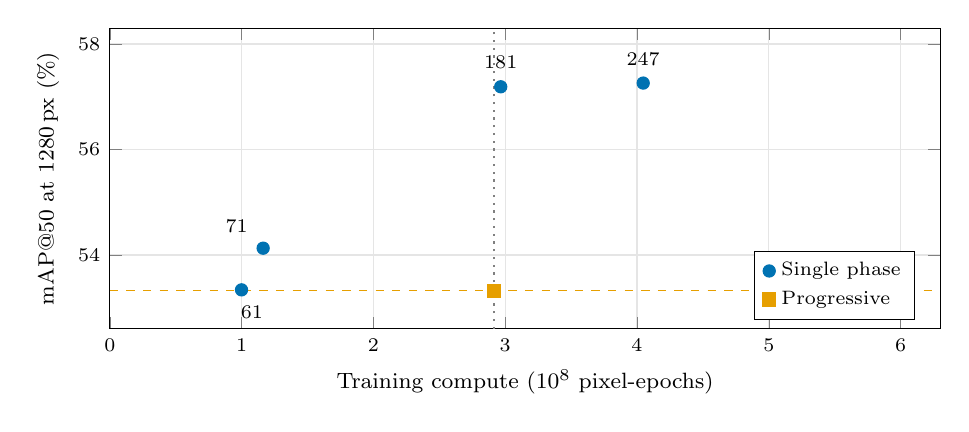
\begin{tikzpicture}
\begin{axis}[
  width=\linewidth, height=5.4cm,
  xlabel={Training compute ($10^8$ pixel-epochs)},
  ylabel={mAP@50 at 1280\,px (\%)},
  xmin=0, xmax=6.3, ymin=52.6, ymax=58.3,
  grid=major, grid style={gray!20},
  legend style={at={(0.97,0.03)}, anchor=south east}, legend cell align=left,
]
\addplot[only marks, mark=*, mark size=2.2pt, color=cSP]
  coordinates {(0.999,53.34) (1.163,54.13) (2.966,57.19) (4.047,57.26)};
\addlegendentry{Single phase}
\addplot[only marks, mark=square*, mark size=2.4pt, color=cProg]
  coordinates {(2.917,53.32)};
\addlegendentry{Progressive}
\draw[cProg, dashed] (axis cs:0,53.32) -- (axis cs:6.3,53.32);
\draw[gray, dotted, thick] (axis cs:2.917,52.6) -- (axis cs:2.917,58.3);
\node[font=\scriptsize, anchor=north west] at (axis cs:0.92,53.22) {61};
\node[font=\scriptsize, anchor=south east] at (axis cs:1.12,54.25) {71};
\node[font=\scriptsize, anchor=south] at (axis cs:2.966,57.35) {181};
\node[font=\scriptsize, anchor=south] at (axis cs:4.047,57.40) {247};
\end{axis}
\end{tikzpicture}
\caption{Accuracy against training compute}
\end{subfigure}\hfill
\begin{subfigure}[t]{0.49\linewidth}
\centering
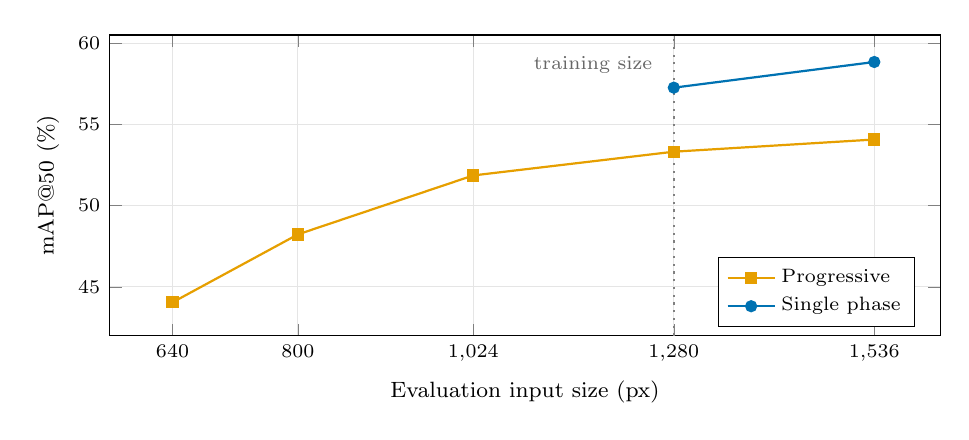
\begin{tikzpicture}
\begin{axis}[
  width=\linewidth, height=5.4cm,
  xlabel={Evaluation input size (px)},
  ylabel={mAP@50 (\%)},
  xtick={640,800,1024,1280,1536},
  xmin=560, xmax=1620, ymin=42, ymax=60.5,
  grid=major, grid style={gray!20},
  legend style={at={(0.97,0.03)}, anchor=south east}, legend cell align=left,
]
\addplot[thick, mark=square*, mark size=1.8pt, color=cProg]
  coordinates {(640,44.05) (800,48.23) (1024,51.86) (1280,53.32) (1536,54.07)};
\addlegendentry{Progressive}
\addplot[thick, mark=*, mark size=1.8pt, color=cSP]
  coordinates {(1280,57.26) (1536,58.84)};
\addlegendentry{Single phase}
\draw[gray, dotted, thick] (axis cs:1280,42) -- (axis cs:1280,60.5);
\node[font=\scriptsize, anchor=north east, text=gray!80!black]
  at (axis cs:1265,59.8) {training size};
\end{axis}
\end{tikzpicture}
\caption{Accuracy against evaluation input size}
\end{subfigure}
\caption{(a)~mAP@50 of single-phase checkpoints after 61, 71 and 181 epochs and of
the best checkpoint (epoch 247), compared with the finished progressive model
(dashed line). The dotted line marks the progressive schedule's compute.
(b)~The same seed-0 models evaluated at different input sizes.}
\label{fig:compute}
\end{figure}

All ten classes improved (Fig.~\ref{fig:perclass}). The largest gain was for
bicycles ($+7.4$ AP@50 at 1280\,px), followed by vans and tricycles ($+4.7$ each);
the smallest were for cars ($+0.8$), which were already above 89 AP, and
awning-tricycles ($+1.3$). Bicycles are among the thinnest objects in the dataset,
which fits prediction P1, but large vehicles such as buses and trucks also gained
more than four points, so per-class results alone do not show that the gain is
concentrated on small objects. Section~\ref{sec:res-size} tests P1 by object size
directly.

\begin{figure}[t]
\centering
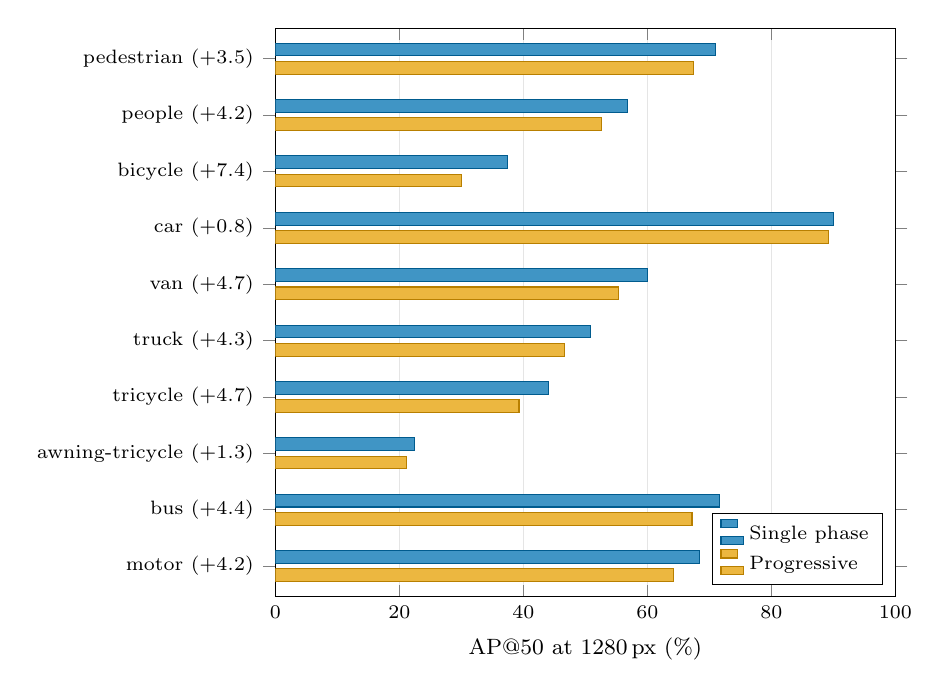
\begin{tikzpicture}
\begin{axis}[
  xbar, width=0.78\linewidth, height=8.8cm, bar width=4.6pt,
  xmin=0, xmax=100, xlabel={AP@50 at 1280\,px (\%)},
  ytick={1,...,10},
  yticklabels={{motor ($+4.2$)}, {bus ($+4.4$)}, {awning-tricycle ($+1.3$)},
               {tricycle ($+4.7$)}, {truck ($+4.3$)}, {van ($+4.7$)},
               {car ($+0.8$)}, {bicycle ($+7.4$)}, {people ($+4.2$)},
               {pedestrian ($+3.5$)}},
  enlarge y limits=0.06, xmajorgrids, grid style={gray!20},
  legend style={at={(0.98,0.02)}, anchor=south east}, legend cell align=left,
  reverse legend,
]
\addplot[fill=cProg!75, draw=cProg!80!black] coordinates {
  (64.2,1) (67.2,2) (21.1,3) (39.3,4) (46.6,5) (55.3,6) (89.2,7) (30.1,8) (52.6,9) (67.5,10)};
\addlegendentry{Progressive}
\addplot[fill=cSP!75, draw=cSP!80!black] coordinates {
  (68.4,1) (71.6,2) (22.4,3) (44.0,4) (50.9,5) (60.0,6) (90.0,7) (37.5,8) (56.8,9) (71.0,10)};
\addlegendentry{Single phase}
\end{axis}
\end{tikzpicture}
\caption{Per-class AP@50 of Baseline-P2 at 1280\,px (seed 0). Numbers in
parentheses give the gain from single-phase training.}
\label{fig:perclass}
\end{figure}

Both models kept improving as the evaluation size grew
(Fig.~\ref{fig:compute}b). The progressive model rose from 44.1\% at 640\,px to
54.1\% at 1536\,px, including a gain of 0.8 points from 1280 to 1536\,px, above its
final training size. The single-phase model gained 1.6 points over the same step.
This is consistent with the sampling argument and with the train--test resolution
effect described by Touvron et al.~\cite{touvron2019fixres}, although neither
explanation is tested directly by these two points.

\subsection{Detection stride}
\label{sec:res-stride}

Table~\ref{tab:stride} compares YOLOv11s with three detection levels and
Baseline-P2, both trained in a single phase at 1280\,px with seed 0.
\tbd[Describe the result once the P3--P5 run is evaluated.] Adding the P2 level
costs 0.49M parameters and raises GFLOPs by 74\% at every input size
(Table~\ref{tab:complexity}), because the stride-4 level operates on a feature map
with four times as many positions as the stride-8 level.

\begin{table}[t]
\centering
\caption{Effect of the stride-4 detection level. Both models were trained in a
single phase at 1280\,px (seed 0).}
\label{tab:stride}
\small
\begin{tabular}{lcccc}
\toprule
 & \multicolumn{2}{c}{1280\,px} & \multicolumn{2}{c}{1536\,px} \\
\cmidrule(lr){2-3}\cmidrule(lr){4-5}
Model & mAP@50 & mAP@50:95 & mAP@50 & mAP@50:95 \\
\midrule
YOLOv11s (P3--P5) & \tbd & \tbd & \tbd & \tbd \\
Baseline-P2       & 57.26 & 34.66 & 58.84 & 35.82 \\
$\Delta$          & \tbd & \tbd & \tbd & \tbd \\
\bottomrule
\end{tabular}
\end{table}

\subsection{Feature modules}
\label{sec:res-modules}

Table~\ref{tab:modules} adds MEIS and FRM to Baseline-P2 under the full
progressive schedule. The change in mAP@50 was $+0.56$ points with seed 0 and
$-0.36$ points with seed 42 at 1280\,px, and $+0.58$ and $-0.34$ points at
1536\,px. Neither difference is significant (Fig.~\ref{fig:forest}): the paired
bootstrap intervals at 1536\,px are $[-0.15, 1.27]$ and $[-1.00, 0.33]$, with
$p=0.11$ and $p=0.41$, and the permutation tests agree ($p=0.12$ and $p=0.37$).
The mAP@50:95 differences, $+0.17$ and $-0.13$ points, are smaller still ($p=0.48$
and $p=0.65$). The same test found the schedule effect of
Section~\ref{sec:res-schedule} with $p<0.001$, so the null result does not come
from an insensitive test. Even on the favourable seed, the interval excludes
improvements larger than about 1.3 points. For this, the modules cost 1.48M
parameters and 18\% more GFLOPs (Table~\ref{tab:complexity}).

\begin{table}[t]
\centering
\caption{Adding MEIS and FRM to Baseline-P2 under the full progressive schedule.
The paired tests are computed at 1536\,px over the 548 validation images.}
\label{tab:modules}
\small
\resizebox{\linewidth}{!}{%
\begin{tabular}{llcccccc}
\toprule
 & & \multicolumn{2}{c}{1280\,px} & \multicolumn{2}{c}{1536\,px} & \multicolumn{2}{c}{Paired test, mAP@50} \\
\cmidrule(lr){3-4}\cmidrule(lr){5-6}\cmidrule(lr){7-8}
Seed & Model & mAP@50 & mAP@50:95 & mAP@50 & mAP@50:95 & 95\% CI & $p$ (bootstrap / perm.) \\
\midrule
0  & Baseline-P2       & 53.32 & 31.47 & 54.07 & 32.01 & & \\
   & + MEIS + FRM      & 53.88 & 31.96 & 54.65 & 32.18 & & \\
   & $\Delta$          & $+0.56$ & $+0.49$ & $+0.58$ & $+0.17$ & $[-0.15,\ +1.27]$ & 0.11 / 0.12 \\
\midrule
42 & Baseline-P2       & 53.60 & 31.51 & 54.26 & 31.91 & & \\
   & + MEIS + FRM      & 53.24 & 31.21 & 53.92 & 31.78 & & \\
   & $\Delta$          & $-0.36$ & $-0.30$ & $-0.34$ & $-0.13$ & $[-1.00,\ +0.33]$ & 0.41 / 0.37 \\
\bottomrule
\end{tabular}%
}
\\[2pt]
\begin{minipage}{\linewidth}\footnotesize
The significance tests re-validate both models with batch size one, which changes
mAP@50 by at most 0.01 points relative to the table.
\end{minipage}
\end{table}

\begin{figure}[t]
\centering
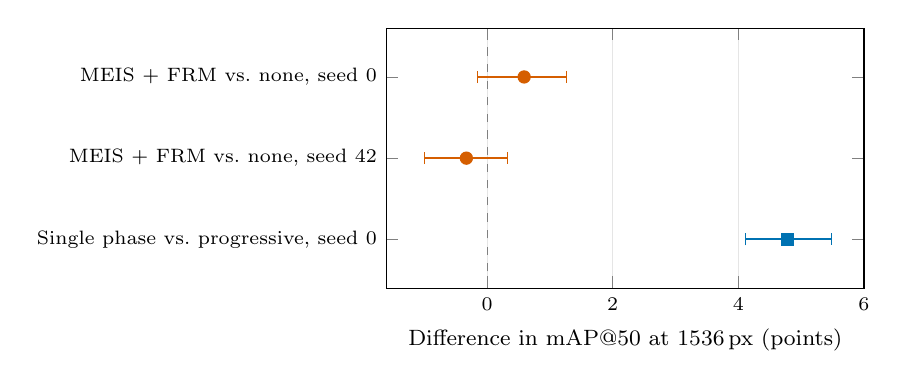
\begin{tikzpicture}
\begin{axis}[
  scale only axis, width=0.5\linewidth, height=3.3cm,
  xlabel={Difference in mAP@50 at 1536\,px (points)},
  xmin=-1.6, xmax=6.0, ymin=0.4, ymax=3.6,
  ytick={1,2,3},
  yticklabels={{Single phase vs.\ progressive, seed 0},
               {MEIS + FRM vs.\ none, seed 42},
               {MEIS + FRM vs.\ none, seed 0}},
  xmajorgrids, grid style={gray!20},
]
\addplot[only marks, mark=*, mark size=2.2pt, color=cMod,
         error bars/.cd, x dir=both, x explicit,
         error bar style={thick, color=cMod}]
  coordinates {(0.59,3) += (0.68,0) -= (0.74,0)
               (-0.33,2) += (0.66,0) -= (0.67,0)};
\addplot[only marks, mark=square*, mark size=2.2pt, color=cSP,
         error bars/.cd, x dir=both, x explicit,
         error bar style={thick, color=cSP}]
  coordinates {(4.78,1) += (0.71,0) -= (0.67,0)};
\draw[gray, dashed] (axis cs:0,0.4) -- (axis cs:0,3.6);
\end{axis}
\end{tikzpicture}
\caption{Paired differences with 95\% bootstrap confidence intervals over the 548
validation images. The module intervals include zero; the schedule interval does
not.}
\label{fig:forest}
\end{figure}

\subsubsection{Factorial ablation of MEIS}
\label{sec:res-factorial}

Table~\ref{tab:factorial} and Fig.~\ref{fig:factorial} separate the two ingredients
of MEIS under the shortened schedule. All four MEIS variants include FRM, and the
reference model has neither module. The model without modules was the most
accurate, and removing either ingredient of MEIS made results slightly better
rather than worse. Averaged over paired same-seed differences at 1280\,px,
multi-scale dilation changed mAP@50 by $-0.20$ points and input-adaptive gating by
$-0.24$ points, each negative in all four pairings, with a negligible interaction
($-0.06$). Full MEIS scored 0.44 points below the plain convolution of equal size.
At 1536\,px the effects pointed the same way ($-0.16$ and $-0.18$ points), in three
of four pairings each. With two seeds, differences of 0.2 points cannot be resolved
statistically; what the ablation does show is that neither ingredient helped.

The module variants trailed the no-module model by 0.6 to 1.0 points in this
75-epoch schedule, whereas under the full schedule the gap was not significant
(Table~\ref{tab:modules}). A plausible reading is that the added blocks slow
optimization early on and, given enough epochs, settle close to an identity mapping
through their residual connections, but we have not tested this directly.

\begin{table}[t]
\centering
\caption{Factorial ablation of MEIS on Baseline-P2 with the 75-epoch progressive
schedule (mean $\pm$ s.d.\ over seeds 0 and 42).}
\label{tab:factorial}
\small
\resizebox{\linewidth}{!}{%
\begin{tabular}{llrcccc}
\toprule
 & & & \multicolumn{2}{c}{1280\,px} & \multicolumn{2}{c}{1536\,px} \\
\cmidrule(lr){4-5}\cmidrule(lr){6-7}
Dilations & Gate & Params (M) & mAP@50 & mAP@50:95 & mAP@50 & mAP@50:95 \\
\midrule
\multicolumn{2}{l}{No module}         &  9.92 & \textbf{51.30} $\pm$ 0.10 & 29.71 & \textbf{51.92} $\pm$ 0.18 & 30.03 \\
(1,1,1) & static                      & 11.25 & 50.71 $\pm$ 0.05 & 29.37 & 51.18 $\pm$ 0.40 & 29.79 \\
(1,2,4) & static                      & 11.25 & 50.54 $\pm$ 0.16 & 29.15 & 51.14 $\pm$ 0.16 & 29.52 \\
(1,1,1) & adaptive                    & 11.40 & 50.50 $\pm$ 0.11 & 29.29 & 51.12 $\pm$ 0.62 & 29.57 \\
(1,2,4) & adaptive (MEIS)             & 11.40 & 50.27 $\pm$ 0.13 & 29.08 & 50.84 $\pm$ 0.47 & 29.26 \\
\midrule
\multicolumn{3}{l}{Dilation (1,2,4) vs.\ (1,1,1)}            & $-0.20$ & & $-0.16$ & \\
\multicolumn{3}{l}{Adaptive vs.\ static gate}                & $-0.24$ & & $-0.18$ & \\
\multicolumn{3}{l}{MEIS vs.\ (1,1,1) with static gate}       & $-0.44$ & & $-0.34$ & \\
\bottomrule
\end{tabular}%
}
\\[2pt]
\begin{minipage}{\linewidth}\footnotesize
All MEIS variants also contain FRM. Effects in the lower block are means of paired
same-seed differences in mAP@50.
\end{minipage}
\end{table}

\begin{figure}[t]
\centering
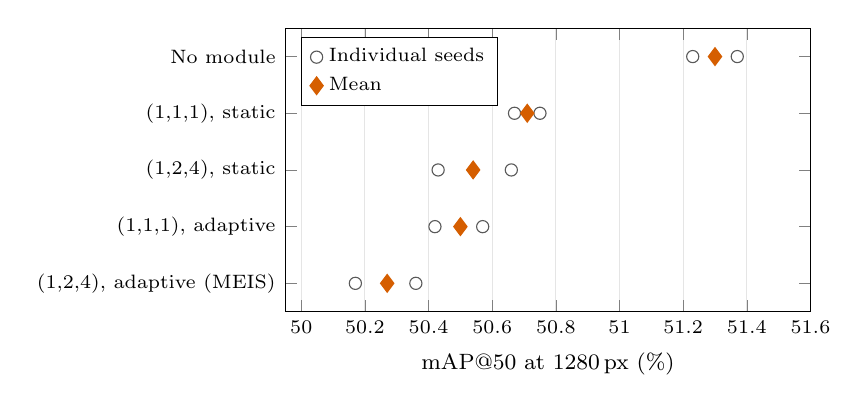
\begin{tikzpicture}
\begin{axis}[
  scale only axis, width=0.55\linewidth, height=3.6cm,
  xlabel={mAP@50 at 1280\,px (\%)},
  xmin=49.95, xmax=51.6, ymin=0.5, ymax=5.5,
  ytick={1,...,5},
  yticklabels={{(1,2,4), adaptive (MEIS)}, {(1,1,1), adaptive},
               {(1,2,4), static}, {(1,1,1), static}, {No module}},
  xmajorgrids, grid style={gray!20},
  legend style={at={(0.03,0.97)}, anchor=north west}, legend cell align=left,
]
\addplot[only marks, mark=o, mark size=2.2pt, color=gray!70!black]
  coordinates {(50.36,1) (50.17,1) (50.57,2) (50.42,2) (50.43,3) (50.66,3)
               (50.67,4) (50.75,4) (51.23,5) (51.37,5)};
\addlegendentry{Individual seeds}
\addplot[only marks, mark=diamond*, mark size=3.2pt, color=cMod]
  coordinates {(50.27,1) (50.50,2) (50.54,3) (50.71,4) (51.30,5)};
\addlegendentry{Mean}
\end{axis}
\end{tikzpicture}
\caption{Factorial ablation of MEIS (Table~\ref{tab:factorial}). Labels give the
branch dilations and the gate type.}
\label{fig:factorial}
\end{figure}

\subsection{Seed variation and image sampling}
\label{sec:res-variance}

The two sources of uncertainty were of different size. For the MEIS and FRM
comparison, the paired difference moved from $+0.58$ to $-0.34$ points at
1536\,px between seeds, a standard deviation of 0.65 points, while the image-level
bootstrap standard error was 0.35 points. Individual models also moved: Baseline-P2
scored 53.32\% and 53.60\% at 1280\,px with the two seeds, and the MEIS model
53.88\% and 53.24\%. Two seeds give only a rough estimate of the seed variance, but
the comparison is enough to show that a single seed would have been misleading
here. Seed 0 alone suggests that the modules add about half a point; seed 42
suggests that they remove a third of one. For effects below one point we would
recommend at least three seeds together with paired tests over the evaluation
images.

\subsection{Accuracy by object size}
\label{sec:res-size}

Table~\ref{tab:size} splits AP@50 by object area using the COCO
ranges~\cite{coco}, computed in original image pixels. \tbd[Describe once the
size-stratified evaluation is available, and state whether the gains concentrate
on small objects as P1 predicts.]

\begin{table}[t]
\centering
\caption{AP@50 at 1280\,px by object area, using COCO area ranges in original
image pixels (seed 0).}
\label{tab:size}
\small
\begin{tabular}{lccc}
\toprule
Model and schedule & Small ($<32^2$) & Medium & Large ($>96^2$) \\
\midrule
Baseline-P2, progressive        & \tbd & \tbd & \tbd \\
Baseline-P2, single phase       & \tbd & \tbd & \tbd \\
YOLOv11s (P3--P5), single phase & \tbd & \tbd & \tbd \\
\bottomrule
\end{tabular}
\end{table}

\subsection{Cross-dataset evaluation on UAVDT}
\label{sec:res-uavdt}

We applied the VisDrone-trained models to UAVDT~\cite{uavdt} without further
training. UAVDT annotates three vehicle classes, which we mapped to the VisDrone
classes car, truck and bus, and Table~\ref{tab:uavdt} lists the results.
\tbd[Describe the frame sampling, the handling of UAVDT ignore regions and of
VisDrone ``van'' predictions, and the results.]
Because UAVDT contains no pedestrians, bicycles or tricycles, this evaluation says
nothing about small non-vehicle objects outside VisDrone.

\begin{table}[t]
\centering
\caption{Zero-shot AP@50 on UAVDT.}
\label{tab:uavdt}
\small
\begin{tabular}{lcccc}
\toprule
Model and schedule & Car & Truck & Bus & mAP@50 \\
\midrule
Baseline-P2, progressive  & \tbd & \tbd & \tbd & \tbd \\
Baseline-P2, single phase & \tbd & \tbd & \tbd & \tbd \\
\bottomrule
\end{tabular}
\end{table}

\subsection{Relation to published results}
\label{sec:res-published}

Published VisDrone results are difficult to compare with each other because
evaluation split, input size, pretraining and inference procedure differ between
papers. Table~\ref{tab:published} shows the problem with the closest related
method. MEIS-YOLO~\cite{meis-yolo} reports 36.0\% AP@50 on the VisDrone-DET2019
test set, for a network trained from scratch at 640\,px, against 34.6\% for its
YOLOv11m baseline. Our models were evaluated on the validation set, start from
COCO weights and use 1280\,px inputs, so the numbers are not on a common scale and
the table should not be read as a ranking. Region-based detectors that process
magnified crops~\cite{clusdet,li2020dmnet,huang2022ufpmp} use several network
passes per image and belong to a different accuracy--cost regime.

\begin{table}[t]
\centering
\caption{Reported VisDrone-DET2019 results with their evaluation protocols. The
rows are not directly comparable.}
\label{tab:published}
\small
\resizebox{\linewidth}{!}{%
\begin{tabular}{llcccc}
\toprule
Method & Split & Input (px) & COCO initialization & AP@50 & Params (M) \\
\midrule
YOLOv11m, as reported in~\cite{meis-yolo} & test & 640  & no  & 34.6 & 20.04 \\
MEIS-YOLO~\cite{meis-yolo}                & test & 640  & no  & 36.0 & 15.04 \\
% TODO: add further methods only with numbers checked against the primary
% source, and fill in split, input size and initialization for each.
\midrule
Baseline-P2, progressive (ours)           & val  & 1280 & yes & 53.3 &  9.92 \\
Baseline-P2, single phase (ours)          & val  & 1280 & yes & 57.3 &  9.92 \\
\bottomrule
\end{tabular}%
}
\end{table}

% ============================================================================
\section{Discussion}
\label{sec:discussion}
% ============================================================================

\subsection{Why did the progressive schedule do worse?}

The two schedules differ in more than resolution. The progressive schedule spends
200 of its 350 epochs at 640 or 800\,px, where Table~\ref{tab:amin} predicts that
objects smaller than 10 to 12.5 pixels cannot be assigned targets even at stride 4.
It also restarts the learning rate with a warm-up at every phase boundary, which
raises the learning rate again after the previous phase has annealed, and it
changes augmentation and loss weights between phases. We did not separate these
factors, so we cannot say how much each contributed; testing a single-resolution
schedule with phase-wise restarts, or a progressive schedule without them, would
answer that. The checkpoint results do rule out one argument for the progressive
schedule, namely faster convergence, because single-phase training matched its
final accuracy after 61 epochs.

\subsection{Why did the modules not help?}

MEIS and FRM act on features that have already been sampled at stride $r$. By the
argument of Section~\ref{sec:sampling}, they can reweight what the backbone
recorded but cannot recover objects that fell between anchor points, and their
residual design lets them stay close to an identity mapping when reweighting does
not help. The factorial ablation fits this reading: the variants differed from
each other by a few tenths of a point, regardless of dilation or gating. Two
caveats apply. Our MEIS block is not the MEIS module of MEIS-YOLO, and the module
experiments used the progressive schedule; whether they behave differently when
trained at 1280\,px throughout remains untested.

\subsection{Practical recommendations}

Three recommendations follow from these experiments. First, train at the input
size that will be used at deployment before trying resolution schedules. Second,
before adding modules, check the finest detection stride against the object size
distribution with Eq.~\eqref{eq:amin}. Third, compare designs with at least two or
three seeds, test paired differences over the evaluation images, and report
training compute alongside accuracy.

\subsection{Limitations}

The study has several limitations. Most configurations were trained with two seeds,
and the single-phase schedule \tbd[with one seed / with two seeds]. VisDrone is
the only dataset with small non-vehicle objects in our evaluation, and UAVDT
covers only vehicles. We studied one detector family at one size, so larger models
and transformer-based detectors may behave differently; we chose YOLOv11s because
it is widely used, has a maintained implementation with pretrained weights, and
is a realistic size for drone platforms. The schedule comparison changes
resolution, learning-rate restarts and augmentation together. The module
experiments used the progressive schedule, and the factorial ablation used a
shortened one. We did not evaluate robustness to motion blur, noise or illumination
changes. Finally, the sampling argument is a heuristic, and FPS figures depend on
the hardware.

% ============================================================================
\section{Conclusion}
\label{sec:conclusion}
% ============================================================================

For YOLOv11s on VisDrone-DET2019, the design decisions that changed small-object
accuracy were the ones that changed how densely objects are sampled. Training at
1280\,px in a single phase outperformed a four-phase progressive schedule by 3.9
points mAP@50 at the same epoch budget and matched its accuracy with a third of the
compute, and the stride-4 detection level \tbd[result]. Edge selection with
adaptive gating and CBAM-style recalibration did not produce measurable gains once
runs were matched and repeated, and neither multi-scale dilation nor adaptive gating
did better than a plain convolution of equal size. These results do not show that
feature modules cannot help small-object detection, but they suggest that such
modules should be compared against baselines trained at the same resolution and
budget, with repeated seeds and paired tests, before their gains are attributed to
the modules themselves.

% ============================================================================
\section*{CRediT authorship contribution statement}
\tbd[Complete with the CRediT roles of each author.]

\section*{Declaration of competing interest}
The authors declare that they have no known competing financial interests or
personal relationships that could have appeared to influence the work reported in
this paper. \tbd[Confirm.]

\section*{Data availability}
VisDrone-DET2019 and UAVDT are publicly available. \tbd[State whether and where the
code, configurations and trained weights will be released.]

\section*{Declaration of generative AI and AI-assisted technologies in the writing process}
\tbd[Complete according to the journal's policy, describing any AI tools used in
preparing the manuscript and the code.]

\section*{Acknowledgements}
The authors thank the VisDrone and UAVDT teams for the benchmarks and the
Ultralytics team for the YOLOv11 implementation.

% ============================================================================
\appendix
\section{Earlier single-seed ablations}
\label{app:early}
% ============================================================================

Before the controlled experiments above, we ran a set of single-seed ablations
with an earlier configuration. It differed from the main experiments in four ways:
the detectors used three detection levels (P3 to P5), module variants did not
receive copied head weights and so started with randomly initialized necks while
the reference neck was pretrained, models were evaluated at 1024\,px, and at most
300 detections were kept per image. Table~\ref{tab:early} reports these runs for
completeness, including the placement of FRM before or after fusion, the residual
blend factor $\alpha$, and two- versus three-level fusion at P4.

\begin{table}[t]
\centering
\caption{Earlier ablations with three detection levels, the full progressive
schedule and evaluation at 1024\,px. One seed per row unless stated.}
\label{tab:early}
\small
\begin{tabular}{lcc}
\toprule
Configuration & mAP@50 & mAP@50:95 \\
\midrule
PANet neck, no module                                    & 49.84 & 29.61 \\
PANet neck + MEIS                                        & 48.15 & 27.96 \\
Weighted fusion (three levels at P4) + MEIS              & 47.91 & 27.96 \\
\quad + FRM after fusion, $\alpha=0.5$ (three runs)      & 48.50 $\pm$ 0.28 & 28.47 $\pm$ 0.27 \\
\quad + FRM before fusion, $\alpha=0.5$                  & 48.02 & 28.15 \\
\quad + FRM after fusion, $\alpha=0.3$                   & 47.90 & 28.13 \\
\quad + FRM after fusion, $\alpha=0.7$                   & 48.91 & 28.62 \\
Weighted fusion (two levels at P4) + MEIS + FRM          & 49.85 & 29.56 \\
\bottomrule
\end{tabular}
\end{table}

No module configuration exceeded the plain PANet neck. Three repeated runs of the
same configuration spanned 48.25\% to 48.80\% mAP@50, and most other differences
among module variants lie within about twice that spread. Two-level fusion scored
1.35 points above the mean of the three-level runs, the opposite of what
simultaneous three-level fusion was designed to achieve, and equalled the
no-module neck. Because the module variants in this configuration started from
randomly initialized necks and each was run once, we do not draw conclusions from
these numbers beyond the absence of a gain over the PANet neck.

\bibliographystyle{elsarticle-num}
\bibliography{references}

\end{document}
